% Definition 3.1: one figure with local and global views.
% The right panel is the defining development for
% kappa=(.85,1.1,.8,1.25,.9,1.15), h=(.4,.38,.45,.36,.43,.34).
% The left panel magnifies its triple P_2,P_3,P_4 (i=3) and rotates its
% positively oriented circle tangent to horizontal. No closure is imposed.
% Compile: pdflatex -output-directory=<scratch> development.tex
\documentclass[border=2pt]{standalone}
\usepackage{amsmath,amssymb,tikz}
\usetikzlibrary{arrows.meta,calc}
\pdfinfoomitdate=1
\pdftrailerid{}
\definecolor{ink}{HTML}{242E2C}
\definecolor{teal}{HTML}{386F79}
\definecolor{gold}{HTML}{A76C27}
\definecolor{berry}{HTML}{99606C}
\definecolor{quiet}{HTML}{9AA3A1}
\begin{document}
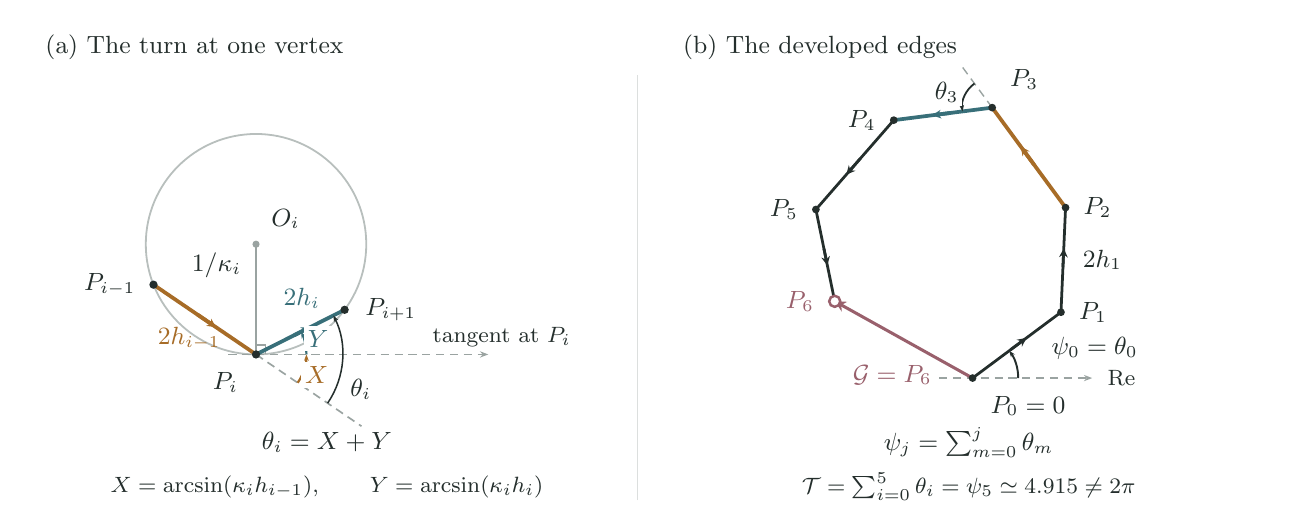
\begin{tikzpicture}[x=1cm,y=1cm,font=\small,text=ink,
    labelbg/.style={fill=white,inner sep=1.5pt}]
\path[use as bounding box] (0,0) rectangle (15.8,6.05);
\node[anchor=west] at (.1,5.8) {(a) The turn at one vertex};
\node[anchor=west] at (8.2,5.8) {(b) The developed edges};
\draw[quiet!35,line width=.4pt] (7.75,.05)--(7.75,5.45);

\coordinate (A) at (1.597794277,2.785937500);\coordinate (B) at (2.900000000,1.900000000);\coordinate (C) at (4.025215979,2.467000000);\coordinate (O) at (2.900000000,3.300000000);
\draw[quiet!70,line width=.65pt] (O) circle[radius=1.4];
\draw[quiet,line width=.6pt,densely dashed,-{Stealth[length=3pt]}] (2.550000000,1.900000000)--(5.850000000,1.900000000);
\draw[quiet,line width=.6pt,densely dashed] (B)--(4.239411601,0.988750000);
\draw[quiet,line width=.6pt] (B)--(O);
\draw[quiet,line width=.5pt] (2.900000000,2.020000000)--(3.020000000,2.020000000)--(3.020000000,1.900000000);
\draw[gold,line width=1.35pt] (1.597794277,2.785937500)--(2.900000000,1.900000000);
\draw[gold,line width=1.35pt,-{Stealth[length=3.2pt,width=3.1pt]}] (2.157742738,2.404984375)--(2.392139768,2.245515625);
\draw[teal,line width=1.35pt] (2.900000000,1.900000000)--(4.025215979,2.467000000);
\draw[teal,line width=1.35pt,-{Stealth[length=3.2pt,width=3.1pt]}] (3.383842871,2.143810000)--(3.586381747,2.245870000);
\draw[gold,line width=.8pt,-{Stealth[length=2.3pt]}] (3.429150262,1.540000000) arc[start angle=-34.228866328,end angle=0,radius=.64];
\draw[teal,line width=.8pt,-{Stealth[length=2.3pt]}] (3.540000000,1.900000000) arc[start angle=0,end angle=26.743683950,radius=.64];
\draw[ink,line width=.55pt,-{Stealth[length=2.3pt]}] (3.809477013,1.281250000) arc[start angle=-34.228866328,end angle=26.743683950,radius=1.10];
\foreach \v in {A,B,C} \fill[ink] (\v) circle[radius=1.5pt];
\fill[quiet] (O) circle[radius=1.3pt];
\node[left=3pt] at (A) {$P_{i-1}$};
\node[below left=3pt] at (B) {$P_i$};
\node[right=4pt] at (C) {$P_{i+1}$};
\node[above right=2pt] at (O) {$O_i$};
\node[labelbg,anchor=east] at (2.77,3.03) {$1/\kappa_i$};
\node[text=gold] at (2.05,2.10) {$2h_{i-1}$};
\node[text=teal] at (3.48,2.61) {$2h_i$};
\node[text=gold,labelbg] at (3.67,1.64) {$X$};
\node[text=teal,labelbg] at (3.69,2.10) {$Y$};
\node[labelbg] at (4.23,1.46) {$\theta_i$};
\node[anchor=west,font=\footnotesize] at (5.02,2.12) {tangent at $P_i$};
\node at (3.8,.78) {$\theta_i=X+Y$};
\node[font=\footnotesize] at (3.8,.22) {$X=\arcsin(\kappa_i h_{i-1}),\qquad Y=\arcsin(\kappa_i h_i)$};
\coordinate (p0) at (12.000000000,1.600000000);
\coordinate (p1) at (13.122851286,2.436184781);
\coordinate (p2) at (13.181161088,3.764905959);
\coordinate (p3) at (12.249062854,5.034479857);
\coordinate (p4) at (10.999158814,4.875294777);
\coordinate (p5) at (10.010421912,3.740647546);
\coordinate (p6) at (10.249388781,2.574888208);
\draw[ink,line width=1.0pt] (12.000000000,1.600000000)--(13.122851286,2.436184781);
\draw[ink,line width=1.0pt,-{Stealth[length=3.2pt,width=3.1pt]}] (12.482826053,1.959559456)--(12.684939285,2.110072717);
\draw[ink,line width=1.0pt] (13.122851286,2.436184781)--(13.181161088,3.764905959);
\draw[ink,line width=1.0pt,-{Stealth[length=3.2pt,width=3.1pt]}] (13.147924501,3.007534888)--(13.158420265,3.246704700);
\draw[gold,line width=1.35pt] (13.181161088,3.764905959)--(12.249062854,5.034479857);
\draw[gold,line width=1.35pt,-{Stealth[length=3.2pt,width=3.1pt]}] (12.780358848,4.310822735)--(12.612581166,4.539346037);
\draw[teal,line width=1.35pt] (12.249062854,5.034479857)--(10.999158814,4.875294777);
\draw[teal,line width=1.35pt,-{Stealth[length=3.2pt,width=3.1pt]}] (11.711604117,4.966030273)--(11.486621390,4.937376958);
\draw[ink,line width=1.0pt] (10.999158814,4.875294777)--(10.010421912,3.740647546);
\draw[ink,line width=1.0pt,-{Stealth[length=3.2pt,width=3.1pt]}] (10.574001946,4.387396468)--(10.396029304,4.183159966);
\draw[ink,line width=1.0pt] (10.010421912,3.740647546)--(10.249388781,2.574888208);
\draw[ink,line width=1.0pt,-{Stealth[length=3.2pt,width=3.1pt]}] (10.113177666,3.239371031)--(10.156191702,3.029534350);
\draw[quiet,line width=.55pt,densely dashed,-{Stealth[length=3pt]}] (11.400000000,1.600000000)--(13.520000000,1.600000000);
\draw[ink,line width=.7pt,-{Stealth[length=2.3pt]}] (12.580000000,1.600000000) arc[start angle=0,end angle=36.674971026,radius=.58];
\node[anchor=west,font=\footnotesize] at (13.59,1.60) {$\operatorname{Re}$};
\node[labelbg] at (13.55,1.98) {$\psi_0=\theta_0$};
\draw[berry,line width=1.1pt,-{Stealth[length=4pt,width=4pt]}] (p0)--(p6);
\node[text=berry,labelbg,align=center] at (10.98,1.64) {$\mathcal G=P_6$};
\node[labelbg] at (13.65,3.10) {$2h_1$};
\draw[quiet,line width=.5pt,densely dashed] (p3)--(11.846633141,5.582613350);
\draw[ink,line width=.65pt,-{Stealth[length=2.3pt]}] (12.024175662,5.340789750) arc[start angle=126.285443197,end angle=187.257993475,radius=.38];
\node[labelbg] at (11.67,5.23) {$\theta_3$};
\foreach \j in {0,...,5} \fill[ink] (p\j) circle[radius=1.4pt];
\draw[berry,fill=white,line width=.9pt] (p6) circle[radius=2pt];
\node[below right=3pt] at (p0) {$P_0=0$};
\node[right=3pt] at (p1) {$P_1$};
\node[right=3pt] at (p2) {$P_2$};
\node[above right=3pt] at (p3) {$P_3$};
\node[left=3pt] at (p4) {$P_4$};
\node[left=3pt] at (p5) {$P_5$};
\node[left=4pt,text=berry] at (p6) {$P_6$};
\node at (11.95,.78) {$\psi_j=\sum_{m=0}^{j}\theta_m$};
\node[font=\footnotesize] at (11.95,.22) {$\mathcal T=\sum_{i=0}^{5}\theta_i=\psi_5\simeq 4.915\ne 2\pi$};
\end{tikzpicture}
\end{document}
